\chapter{Cadre scientifique et probl\'ematique de recherche}
\label{chap:cadre-recherche}

\section{Introduction}

Ce projet d'\'et\'e a \'et\'e men\'e dans un cadre acad\'emique et autonome. Ce
chapitre en \'etablit le cadre scientifique \`a travers une \'etude du contexte,
des travaux existants et des limites de validit\'e qui structurent la recherche.

L'objectif est de d\'efinir pr\'ecis\'ement le probl\`eme trait\'e par le prototype
\emph{IoT Network-Flow Intrusion Detection}. Nous pr\'esentons d'abord le cadre de
la d\'etection d'intrusions dans l'Internet des objets, puis le jeu de donn\'ees
retenu et les principales approches d'apprentissage automatique. Cette analyse
permet ensuite de formuler la probl\'ematique, de d\'elimiter la contribution du
projet et d'exposer la m\'ethodologie suivie.

\section{Contexte scientifique}

\subsection{D\'etection d'intrusions dans les environnements IoT}

Un syst\`eme de d\'etection et de pr\'evention d'intrusions observe des \'ev\'enements
sur un h\^ote ou un r\'eseau afin d'identifier des activit\'es susceptibles de
compromettre la confidentialit\'e, l'int\'egrit\'e ou la disponibilit\'e des
ressources \citep{scarfone_guide_2007}. Dans un environnement IoT, cette fonction
est rendue plus difficile par l'h\'et\'erog\'en\'eit\'e des appareils, des protocoles
et des capacit\'es mat\'erielles. La litt\'erature distingue notamment les m\'ethodes
selon la source des donn\'ees, la strat\'egie de d\'etection et le positionnement du
d\'etecteur dans l'architecture IoT \citep{zarpelao_survey_2017}.

Le pr\'esent projet se limite aux observations agr\'eg\'ees par flux r\'eseau. Une
observation d\'ecrit les deux sens d'une communication au moyen de compteurs, de
dur\'ees, de statistiques de paquets et d'attributs protocolaires. Cette
repr\'esentation est plus compacte qu'une analyse du contenu de chaque paquet,
mais sa valeur d\'epend directement de la d\'efinition et de la reproductibilit\'e
de l'extracteur. Des outils tels que NFStream permettent de construire des
mesures de flux programmables; ils ne garantissent toutefois pas, \`a eux seuls,
l'\'equivalence avec les variables d'un jeu de donn\'ees produit par un autre
extracteur \citep{aouini_nfstream_2022}.

La figure~\ref{fig:nist-passive-idps} fournit un rep\`ere architectural pour
l'observation passive du trafic. Elle illustre plusieurs points de copie, des
capteurs IDPS et un r\'eseau de gestion s\'epar\'e. Elle n'est pas pr\'esent\'ee comme
l'architecture du prototype: elle sert uniquement \`a situer le principe de
collecte hors bande d\'ecrit par le NIST.

\begin{figure}[htbp]
  \centering
  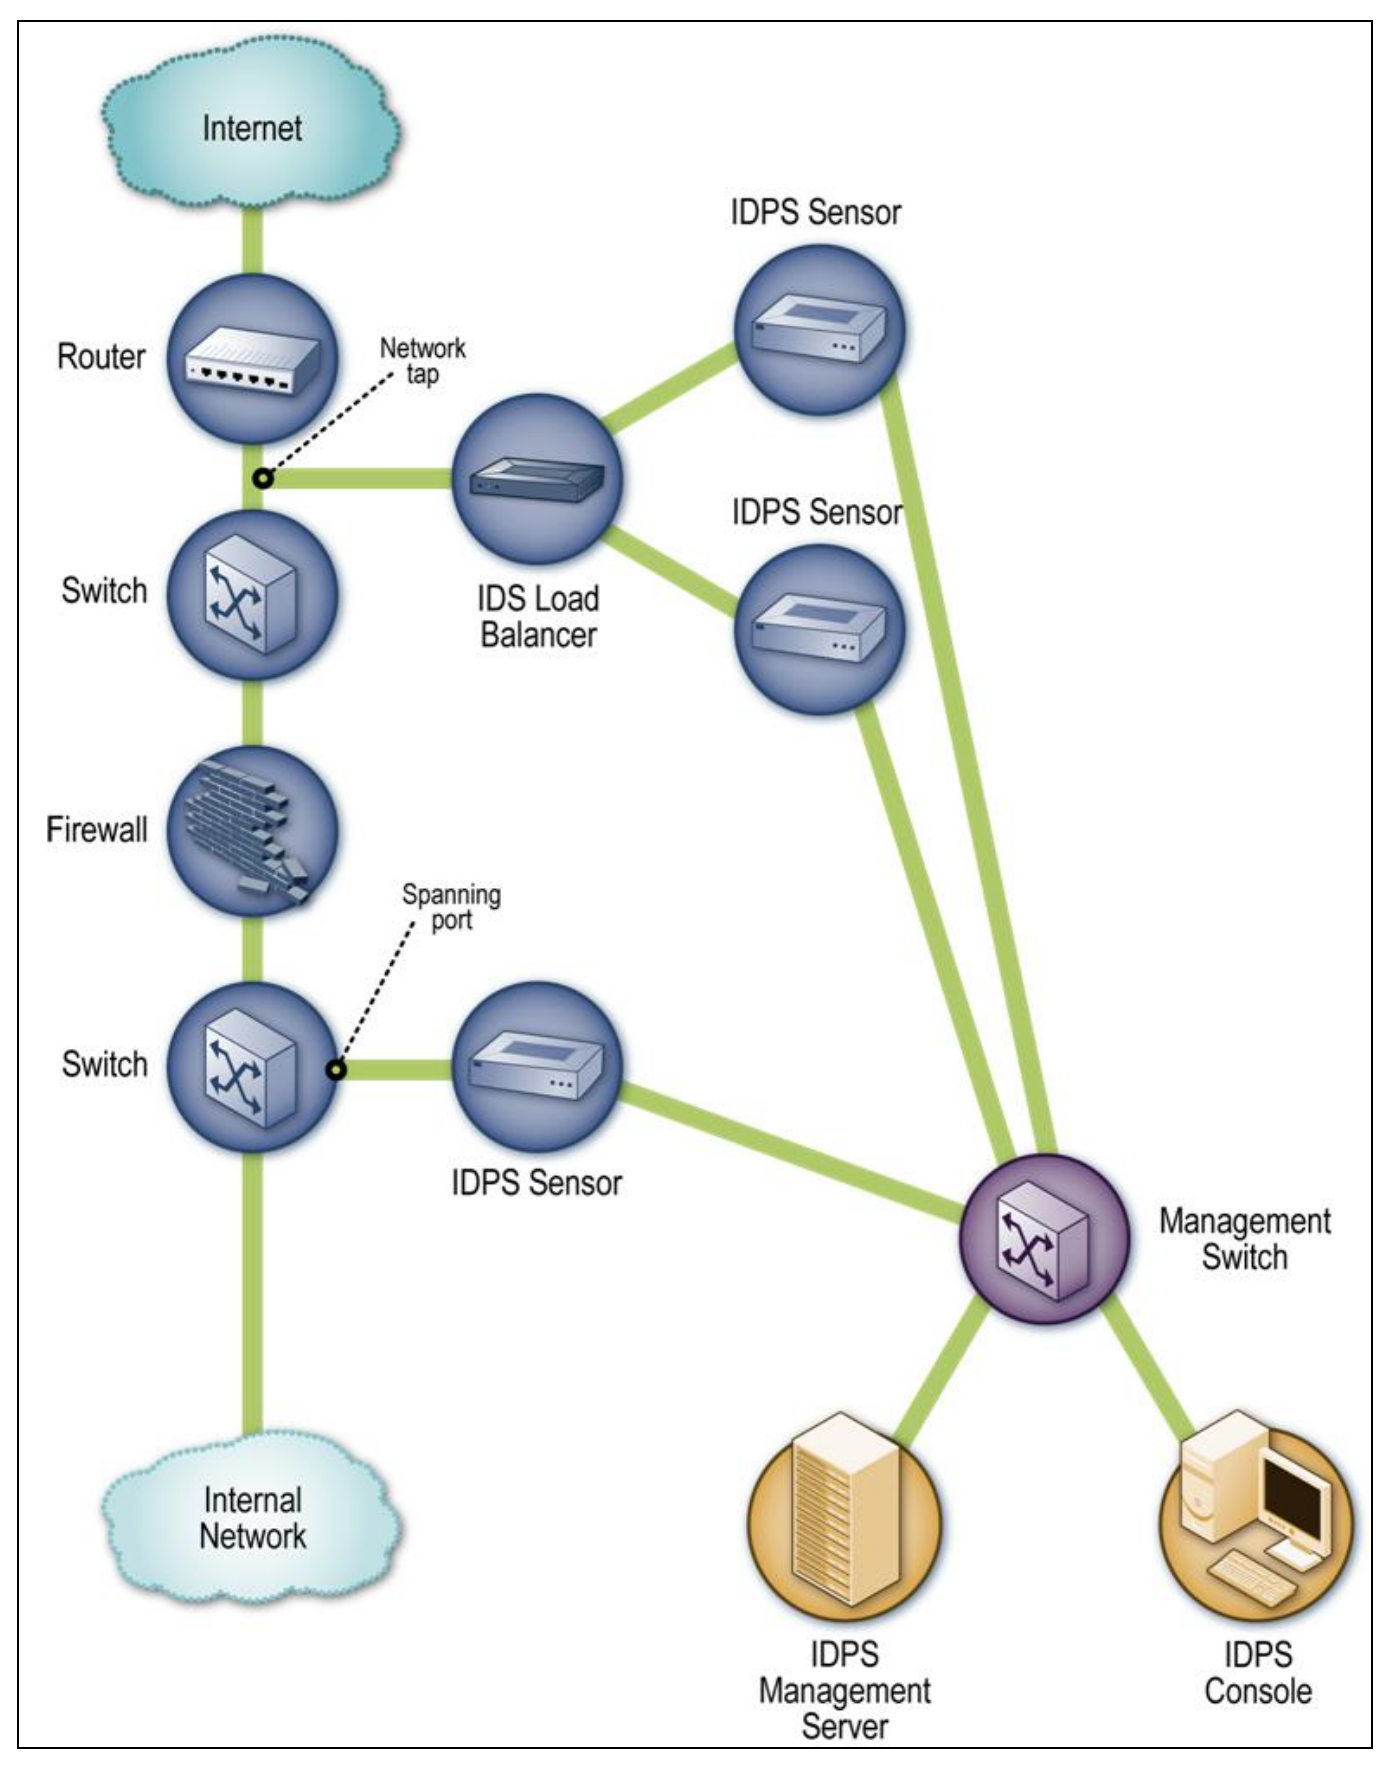
\includegraphics[width=0.58\textwidth]{assets/external/nist-passive-idps-architecture.png}
  \caption[Architecture de r\'ef\'erence d'un IDPS r\'eseau passif]{Architecture de
    r\'ef\'erence d'un IDPS r\'eseau passif. Source: figure~4-3 de
    \citet{scarfone_guide_2007}.}
  \label{fig:nist-passive-idps}
\end{figure}

\subsection{Jeu de donn\'ees RT-IoT2022}

RT-IoT2022 a \'et\'e choisi comme support exp\'erimental. La notice UCI le pr\'esente
comme un jeu de donn\'ees tabulaire multivari\'e consacr\'e au trafic IoT et publie
123\,117 observations comportant 83 variables \citep{b_s_rt-iot2022_2023}. Le
travail associ\'e \'etudie \'egalement un autoencodeur quantifi\'e destin\'e \`a la
d\'etection d'anomalies sur des dispositifs aux ressources contraintes
\citep{sharmila_quantized_2023}.

Dans ce projet, les faits exp\'erimentaux proviennent du fichier CSV officiel
contr\^ol\'e par somme SHA-256, et non d'une reconstruction de la description en
ligne. L'audit local confirme 123\,117 lignes, 83 variables de mod\`ele et douze
\'etiquettes observ\'ees: trois classes de trafic normal et neuf familles
d'attaque. Il rel\`eve \'egalement 5\,202 vecteurs de caract\'eristiques dupliqu\'es
et une forte concentration de la classe \texttt{DOS\_SYN\_Hping}. Ces propri\'et\'es
imposent une d\'eduplication avant la s\'eparation des donn\'ees et une lecture
prudente des scores agr\'eg\'es.

\begin{table}[htbp]
  \centering
  \caption{R\'esultats de l'audit local du fichier RT-IoT2022 contr\^ol\'e}
  \label{tab:rt-iot2022-audit}
  \renewcommand{\arraystretch}{1.20}
  \rowcolors{2}{EmeraldWash}{white}
  \begin{tabularx}{0.88\textwidth}{@{}Y>{\raggedleft\arraybackslash\bfseries\color{PremiumEmerald}}p{0.24\textwidth}@{}}
    \ReportTableHeader{Propri\'et\'e v\'erifi\'ee}{Valeur observ\'ee}
    Observations sources & 123\,117 \\
    Variables utilis\'ees par les mod\`eles & 83 \\
    \'Etiquettes observ\'ees & 12 \\
    Observations normales & 12\,507 \\
    Observations d'attaque & 110\,610 \\
    Vecteurs de caract\'eristiques dupliqu\'es & 5\,202 \\
  \end{tabularx}
  \rowcolors{2}{}{}
\end{table}

La provenance de l'extraction constitue une limite importante. Les sources
publiques ne donnent pas une description suffisamment coh\'erente des outils,
unit\'es, temporisations et r\`egles directionnelles pour affirmer qu'un nouveau
flux extrait localement est num\'eriquement compatible avec les 83 variables
publi\'ees. En outre, le tableau ne contient pas d'identifiant fiable de session,
d'appareil ou de temps permettant une s\'eparation chronologique ou group\'ee.

Une validation externe demanderait donc une cha\^ine de capture document\'ee et
reproductible. La figure~\ref{fig:nist-iot-capture} montre un exemple officiel
d'environnement de capture pour appareils IoT filaires et sans fil. Il s'agit
d'une architecture m\'ethodologique de r\'ef\'erence, et non de l'environnement
ayant produit RT-IoT2022 ni d'un composant actuellement d\'eploy\'e par ce projet.

\begin{figure}[htbp]
  \centering
  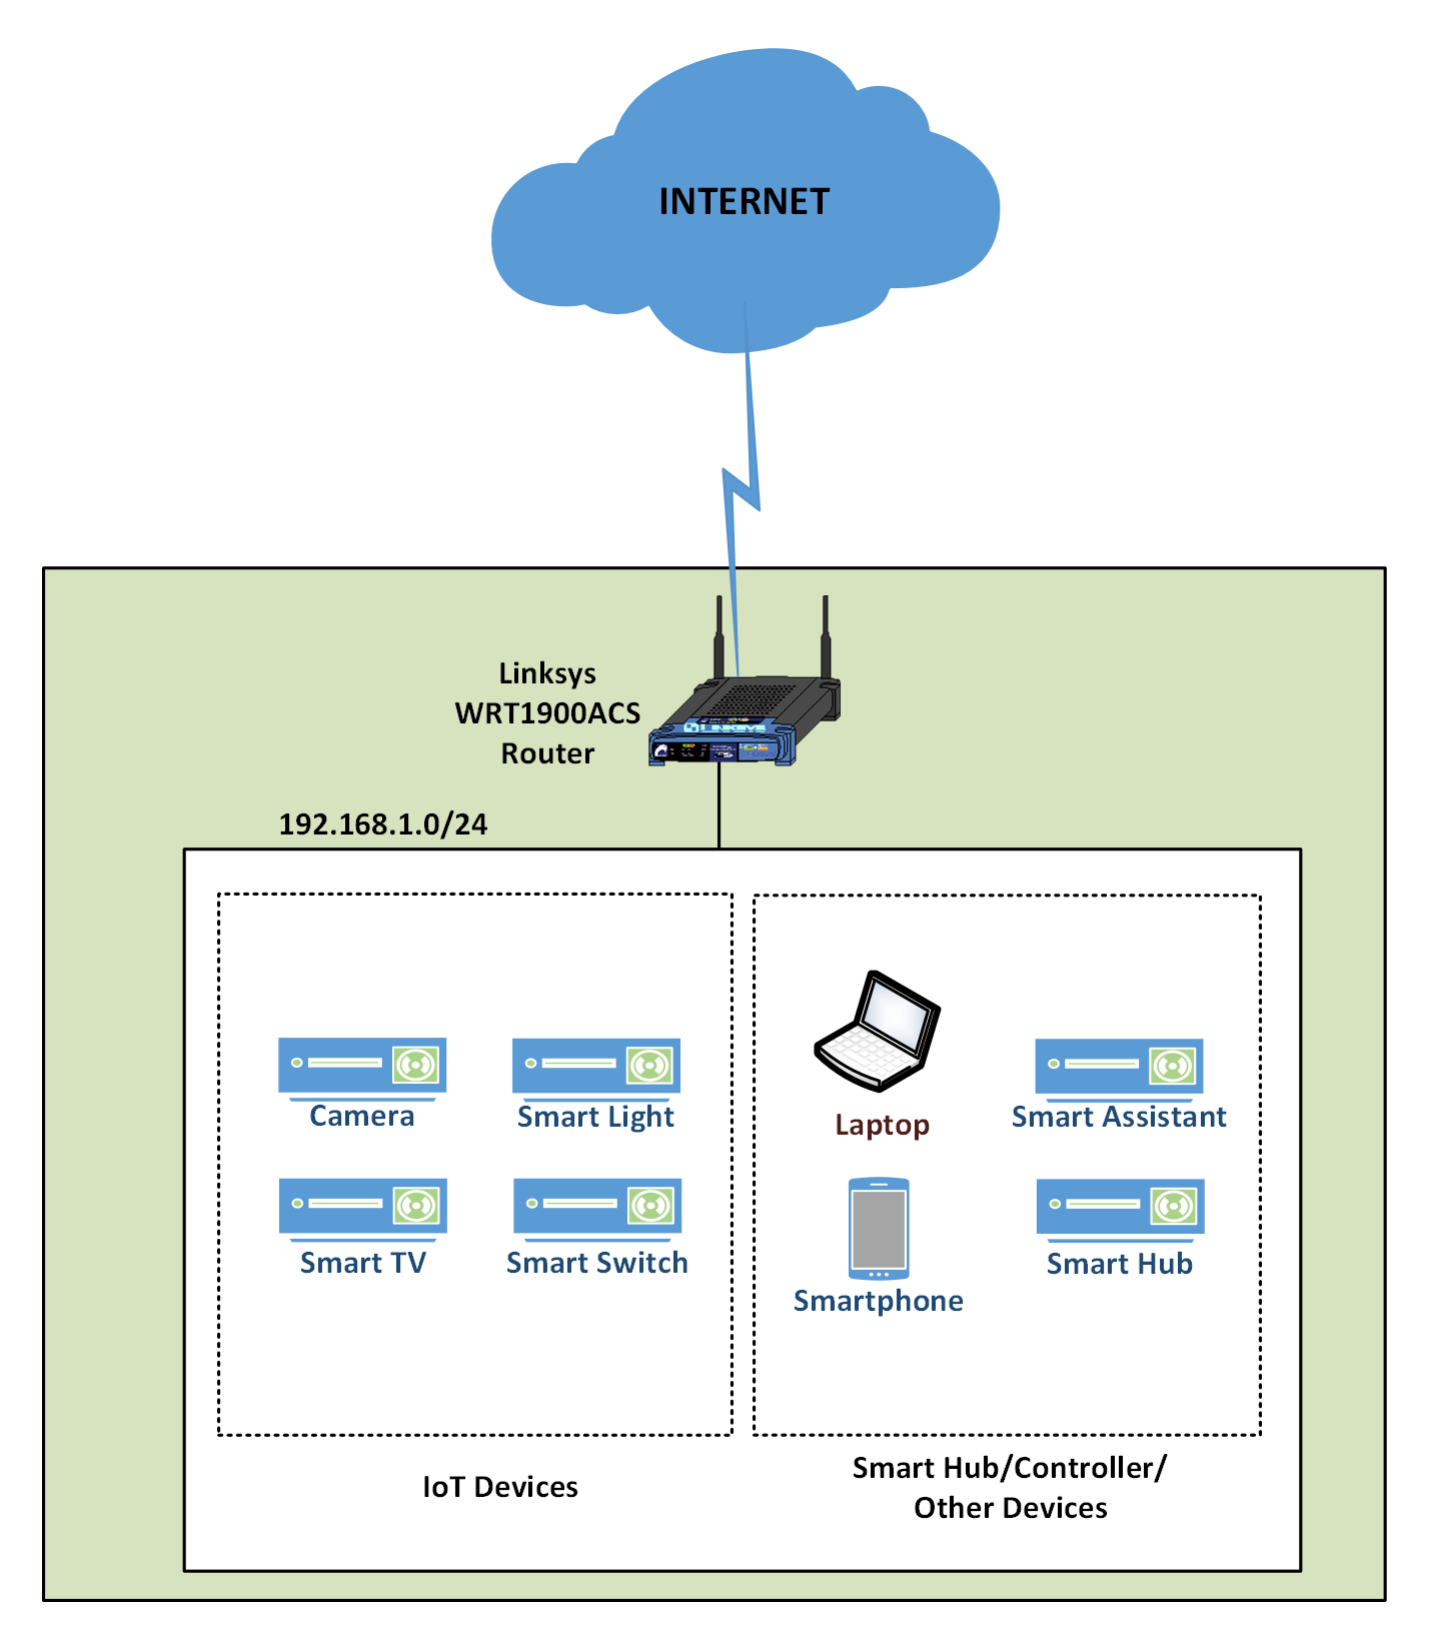
\includegraphics[width=0.64\textwidth]{assets/external/nist-iot-capture-architecture.png}
  \caption[Exemple d'architecture de capture IoT]{Exemple d'architecture de
    capture IoT. Source: figure~4 de \citet{watrobski_methodology_2025}.}
  \label{fig:nist-iot-capture}
\end{figure}

\section{Analyse des approches existantes}

\subsection{D\'etection par signatures et d\'etection statistique}

La d\'etection par signatures recherche des motifs connus. Elle offre une
justification directe lorsqu'une r\`egle correspond, mais reste d\'ependante de la
couverture et de la mise \`a jour de cette base de r\`egles. La d\'etection
statistique ou par apprentissage cherche au contraire des r\'egularit\'es dans les
donn\'ees. Elle peut reconna\^itre des configurations plus complexes, au prix
d'une d\'ependance forte envers les donn\'ees d'entra\^inement et le contexte de
collecte. Ces familles sont compl\'ementaires; le laboratoire Suricata du projet
est donc consid\'er\'e comme une source de preuves par signatures distincte des
pr\'edictions du mod\`ele RT-IoT2022.

\subsection{Classification supervis\'ee des flux}

Le banc d'essai du projet compare quatre familles disponibles dans
Scikit-learn \citep{pedregosa_scikit-learn_2011}: r\'egression logistique, arbre
de d\'ecision, for\^et al\'eatoire et gradient boosting par histogrammes. Les for\^ets
al\'eatoires combinent plusieurs arbres construits avec de l'al\'ea afin de r\'eduire
la variance \citep{breiman_random_2001}; le gradient boosting construit
progressivement un mod\`ele additif optimisant une fonction de perte
\citep{friedman_greedy_2001}.

L'architecture retenue est une cascade \`a deux \'etages. Le premier classifieur
s\'epare les flux normaux des attaques. Le second n'est sollicit\'e que pour les
flux class\'es comme attaques et attribue alors une famille. Cette s\'eparation
refl\`ete le chemin d'inf\'erence r\'eel: une attaque manqu\'ee par le premier
\'etage ne peut recevoir aucune famille au second. Par cons\'equent, l'\'evaluation
doit publier \`a la fois les r\'esultats de chaque \'etage et ceux de la cascade
compl\`ete.

\subsection{Limites des validations usuelles}

Une erreur de protocole peut produire un score optimiste sans am\'eliorer le
syst\`eme r\'eel. La fuite de donn\'ees appara\^it lorsqu'une information indisponible
au moment de la pr\'ediction influence l'entra\^inement ou la s\'election du mod\`ele
\citep{kaufman_leakage_2012}. Dans le cas pr\'esent, le pr\'etraitement doit donc
\^etre ajust\'e uniquement sur l'ensemble d'entra\^inement, et les doublons exacts
doivent \^etre trait\'es avant la partition.

La g\'en\'eralisation entre environnements est une seconde menace. Une \'etude
inter-jeux de donn\'ees rapporte que des classifieurs presque parfaits dans leur
jeu d'origine peuvent perdre fortement en performance lorsqu'ils sont appliqu\'es
\`a une autre collecte \citep{cantone_machine_2024}. Ce r\'esultat ne mesure pas
directement RT-IoT2022, mais il interdit d'assimiler une validation al\'eatoire sur
un seul fichier \`a une validation sur un r\'eseau de d\'eploiement.

Enfin, l'exactitude seule est insuffisante lorsque les classes sont
d\'es\'equilibr\'ees. Le projet privil\'egie donc la macro-F1, les matrices de
confusion, le support et le rappel par classe, ainsi que le taux de faux positifs.
Ces mesures r\'epondent \`a des aspects diff\'erents d'une t\^ache de classification
\citep{sokolova_systematic_2009}. Les scores probabilistes sont calibr\'es sur des
donn\'ees de validation s\'epar\'ees, puisque la qualit\'e du classement et celle des
probabilit\'es constituent deux propri\'et\'es distinctes
\citep{niculescu-mizil_predicting_2005}.

\section{Probl\'ematique et questions de recherche}

La probl\'ematique retenue est la suivante:

\begin{quote}
Comment construire un prototype reproductible capable de classifier des flux
RT-IoT2022 en deux \'etapes, de conserver les preuves de ses d\'ecisions et de
signaler honn\^etement les limites qui s\'eparent une bonne performance interne
d'une validation sur un r\'eseau IoT r\'eel?
\end{quote}

Cette probl\'ematique se d\'ecompose en quatre questions:

\begin{enumerate}
  \item comment garantir la provenance, le sch\'ema et l'ordre des variables
        utilis\'ees pendant l'entra\^inement et l'inf\'erence;
  \item quelle combinaison de d\'etecteur binaire et de classifieur de familles
        offre le meilleur compromis mesur\'e sur le protocole d\'eclar\'e;
  \item quelles erreurs sont introduites par chacun des deux \'etages et par la
        cascade compl\`ete;
  \item quelles preuves suppl\'ementaires seraient n\'ecessaires avant toute
        affirmation de d\'etection sur un r\'eseau externe ou en temps r\'eel.
\end{enumerate}

\section{Solution propos\'ee et p\'erim\`etre}

La solution propos\'ee est un prototype de recherche reproductible compos\'e de
quatre cha\^ines coh\'erentes. La premi\`ere pr\'epare et contr\^ole le jeu de donn\'ees,
supprime les doublons selon une politique explicite et produit un sch\'ema
versionn\'e. La deuxi\`eme entra\^ine plusieurs candidats, s\'electionne les mod\`eles
sur la validation et r\'eserve le test \`a l'estimation finale. La troisi\`eme sert
la cascade au moyen d'une API, persiste les observations, pr\'edictions et alertes,
puis transmet les \'ev\'enements apr\`es validation. La quatri\`eme fournit une
interface d'investigation, des explications locales et des indicateurs de sant\'e
du mod\`ele.

Le p\'erim\`etre doit rester explicite. Le syst\`eme classifie des enregistrements
de flux valid\'es et rejoue des observations enregistr\'ees. Il ne prouve pas que
le mod\`ele RT-IoT2022 est compatible avec un flux captur\'e par NFStream, ni qu'il
se g\'en\'eralise \`a un autre r\'eseau. Le laboratoire Suricata analyse de vrais
paquets dans un environnement isol\'e, mais ses alertes de signatures ne sont pas
des pr\'edictions du mod\`ele. Ces fronti\`eres emp\^echent de transformer une preuve
d'ing\'enierie en affirmation scientifique non mesur\'ee.

L'interface qui restitue ces limites et les preuves d'\'evaluation est pr\'esent\'ee
avec les autres vues principales au chapitre~\ref{chap:realisation}.

\section{D\'emarche de recherche}

\subsection{Mode de d\'eveloppement}

Le d\'eveloppement suit une d\'emarche incr\'ementale guid\'ee par les preuves.
Chaque incr\'ement part d'un contrat ou d'une limite explicite, ajoute les tests
correspondants, impl\'emente le comportement puis produit un artefact
v\'erifiable. L'historique du d\'ep\^ot atteste cette progression depuis la
pr\'eparation des donn\'ees jusqu'à l'ingestion, à la supervision et au
laboratoire isol\'e. Cette organisation ne pr\'etend pas appliquer un cadre Scrum
ou un calendrier d'entreprise qui n'ont pas exist\'e.

\subsection{Phases de recherche}

La conduite du projet est organis\'ee en phases tra\c{c}ables:

\begin{enumerate}
  \item audit des sources scientifiques, du fichier RT-IoT2022 et de son sch\'ema;
  \item pr\'eparation reproductible des donn\'ees et d\'efinition du protocole
        d'\'evaluation;
  \item comparaison des candidats, calibration, analyse des erreurs et promotion
        atomique des artefacts;
  \item conception de l'API, de la persistance et de l'ingestion durable,
        puis r\'ealisation de l'interface d'investigation;
  \item tests unitaires, tests d'int\'egration, validation des artefacts et
        constitution d'un paquet de preuves reproductible;
  \item identification des travaux non encore valid\'es: collecte native
        NFStream, s\'eparation par session ou par temps, validation externe et
        mesure sur le mat\'eriel cible.
\end{enumerate}

Cette organisation constitue une d\'emarche de recherche v\'erifiable. Chaque
phase produit un artefact contr\^olable:
manifestes et sommes de contr\^ole, rapports d'\'evaluation, mod\`eles versionn\'es,
tests automatis\'es, documentation d'architecture ou preuves d'ex\'ecution.

Le carnet ex\'ecut\'e fournit une trace lisible de la comparaison des candidats.
La figure~\ref{fig:notebook-model-comparison} reproduit directement sa section
de comparaison, sans ressaisir ni recalculer les valeurs dans le rapport.

\begin{figure}[htbp]
  \centering
  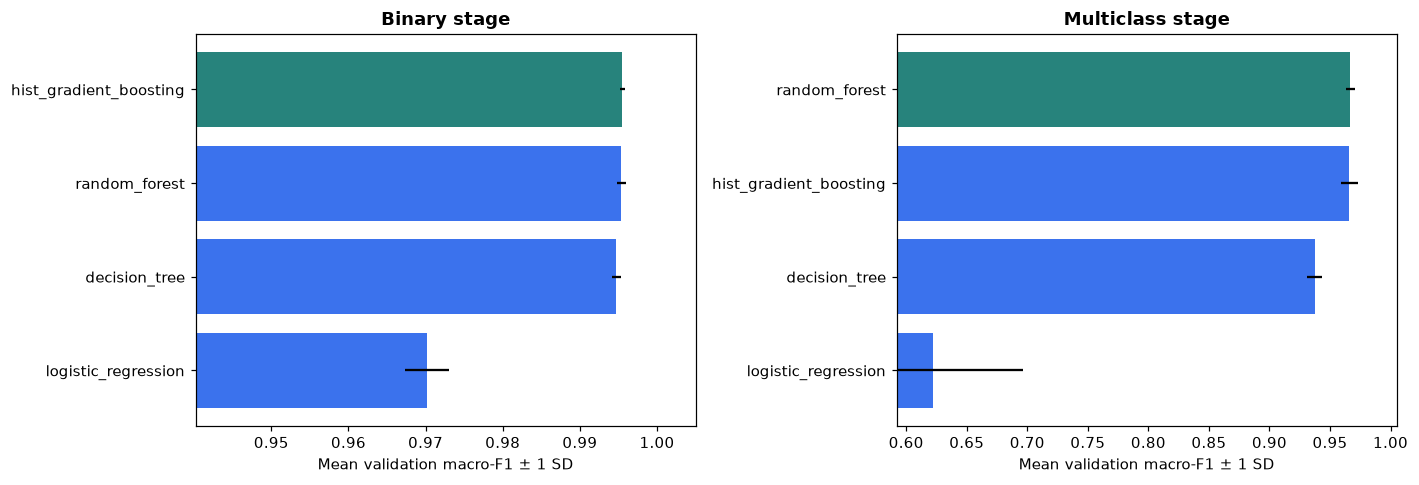
\includegraphics[width=\textwidth]{assets/screenshots/notebook-model-comparison.png}
  \caption{Comparaison des mod\`eles dans le carnet de recherche ex\'ecut\'e}
  \label{fig:notebook-model-comparison}
\end{figure}

La chronologie de la figure~\ref{fig:gantt-realisation} est r\'etrospective.
Ses bornes proviennent de l'historique Git: du premier commit dat\'e du
23~juillet~2026 au paquet de preuves et au carnet ex\'ecut\'e finalis\'es le
25~ao\^ut~2026. Elle ne constitue pas un planning pr\'evisionnel: elle documente
la progression observ\'ee.

\begin{figure}[htbp]
  \centering
  \begin{ganttchart}[
      x unit=0.245cm,
      y unit title=0.58cm,
      y unit chart=0.68cm,
      vgrid={*{34}{draw=SoftRule!55}},
      hgrid=false,
      title/.style={draw=none,fill=EmeraldMist},
      title label font=\scriptsize\bfseries\color{PremiumEmerald},
      bar/.append style={draw=PremiumEmerald,fill=Emerald!78,rounded corners=1.2pt},
      bar height=0.48,
      bar label font=\scriptsize\color{Charcoal},
      bar label node/.append style={align=right,text width=4.75cm},
      group label font=\scriptsize,
      link/.style={-Latex,draw=MutedInk},
      canvas/.append style={draw=none}
    ]{1}{34}
    \gantttitle{23 Jul}{7}
    \gantttitle{30 Jul}{7}
    \gantttitle{06 Aug}{7}
    \gantttitle{13 Aug}{7}
    \gantttitle{20 Aug}{6} \\
    \ganttbar{Foundations and experiments}{1}{13} \\
    \ganttbar{API and dashboard}{13}{14} \\
    \ganttbar{Ingestion, authentication, and security}{16}{20} \\
    \ganttbar{User experience and operations}{20}{30} \\
    \ganttbar{Isolated network laboratory}{29}{30} \\
    \ganttbar{Evidence package and executed notebook}{33}{34}
  \end{ganttchart}
  \caption{Chronologie de r\'ealisation fond\'ee sur les dates de l'historique Git}
  \label{fig:gantt-realisation}
\end{figure}

\section{Conclusion}

Ce chapitre a situ\'e le projet dans le domaine de la d\'etection d'intrusions sur
flux IoT et a d\'efini un cadre scientifique adapt\'e \`a un travail autonome.
L'analyse de RT-IoT2022 et des
travaux existants justifie une cascade supervis\'ee reproductible, tout en
montrant que les scores obtenus sur un seul jeu de donn\'ees ne constituent pas
une validation de d\'eploiement. La probl\'ematique, le p\'erim\`etre et la d\'emarche
ainsi d\'efinis serviront de base \`a la sp\'ecification des besoins du syst\`eme au
chapitre suivant.
